% !TeX spellcheck = fr_FR
\chapter{Chapitre 4 : Ensemble de données}
\label{chap:4}

L'ensemble de données est séparé en deux parties; la première est destinée à l'entrainement des modèles, puis la seconde, qui est destinée à les évaluer.

Dans les deux parties, les données sont des fichiers audio mono au format wav, échantillonnés à 44.1[kHz] et encodés sur 16 bits signés. Ainsi, on respecte le théorème d'échantillonnage de Nyquist-Shanon \parencite{noauthor_theoreme_2021} et on évite le problème du repliement de spectre lors de l'analyse dans le monde des fréquences.

Nous allons tirer plusieurs extraits de ces fichiers audio qui seront nos exemples pour les différents modèles. Pour ce faire, nous allons définir une taille de fenêtre qui représentera la taille de notre exemple. Par exemple une fenêtre de 2048 échantillons, ce qui représente une résolution temporelle de \textasciitilde0.046[s] pour un signal échantillonné à 44.1[kHz].

J'ai décidé de représenter les accords à trois sons mineurs et majeurs qui se jouent sur les deux cordes les plus graves, à savoir la corde de E et de A et jusqu'à la $12^\text{ème}$ frette (case de la guitare) non incluse. Ce qui représente un total de 24 accords par corde. Les notes quant à elles sont toutes représentées.

\section{Regroupement des classes}
\label{sec:4.1}

Afin de ne pas avoir trop de classes en sortie du modèle, j'ai décidé de regrouper les classes par notes et par accords, quelle que soit l'octave dans laquelle ils se trouvent. Par exemple la classe Emaj contient le Emaj avec la basse E à \textasciitilde82[Hz] ainsi que l'accord Emaj avec la basse E à \textasciitilde164[Hz]. Même si l'accord ne se trouve pas dans la même octave, il sera classifié comme un Emaj. Pareils pour les notes, même si elles ne sont pas dans la même octave, par exemple un A à 110[Hz] et un A à 220[Hz], elles seront classifiées comme A.

J'ai pris cette décision parce que si j'avais fait une classification par octave (Amaj1 = Amaj dans la première octave, Amaj2 = Amaj dans la deuxième octave, etc.) je me serais retrouvé avec beaucoup de classes en sortie du modèle. À savoir $8 * 2$ accords (mineur, majeur) dans la première octave plus $9 * 2$ accords dans la deuxième, ce qui correspond donc à $34$ classes pour les accords mineurs et majeurs. À cela s'ajoutent les $4 * 12$ notes (chaque note est présente sur 4 octaves) pour un total de $82$ classes. En regroupant de la sorte, j'ai réduit le nombre de classes à $36$.

\section{Matériel utilisé}
\label{sec:4.2}

Pour enregistrer les fichiers, j'ai utilisé une carte son usb Roland Rubix24. Cette carte son est intéressante, car elle est entièrement blindée, ce qui réduit les interférences qui pourront se propager dans le signal et produit un bruit extrêmement faible de l'entrée à la sortie du signal. Elle m'a donc permis d'enregistrer des sons clairs et détaillés avec une excellente qualité sonore. Il est important pour le bon entrainement des modèles que l'ensemble de données soit le plus parfait et représentatif du problème que l'on veut résoudre.

Avant l'utilisation de cette carte son externe, j'avais enregistré un premier ensemble de données avec la carte son interne de mon ordinateur. Mais les signaux enregistrés à l'aide de cette carte son étaient fortement bruités, un bruit de souffle constant y était présent. On appelle ce phénomène "Bruit Blanc". J'ai constaté une nette amélioration de la précision des différents modèles après avoir enregistré le nouvel ensemble de données en utilisant la carte son externe (carte son spécialisée).

\section{Enregistrement des accords à trois sons}
\label{sec:4.3}

Dans cette partie, nous allons détailler la structure des fichiers audio qui représentent les différents accords à trois sons. Par structure, j'entends l'organisation des accords dans les fichiers et les différentes attaques que j'ai effectuées afin d'avoir un ensemble de données le plus représentatif de la réalité. Un fichier audio contiendra uniquement l'accord qui le concerne (par exemple Amaj1.wav contient uniquement Amaj).

\subsection{Ensemble de données d'entrainement}
\label{sec:4.4}

Le fichier va contenir huit fois le même accord, mais jouer avec des attaques et des manières différentes. Les deux premières fois, je vais jouer l'accord en pinçant les cordes avec les doigts, cela va me permettre de générer une attaque plutôt douce et longue dans la durée. Ensuite, les deux accords suivants sont joués en grattant les cordes avec la main, cela va produire une attaque légèrement plus brute et plus courte. Ensuite, deux accords sont joués avec le plectre (médiator) en grattant les cordes d'une manière sèche. Cela va produire une attaque très forte et très courte. Puis les deux derniers accords sont joués au plectre en arpège legato (toutes les notes de l'accord à la suite). Cette technique va décomposer l'accord en désynchronisant les différentes notes et donc signaux qui le composent.

\subsection{Ensemble de données de validation}
\label{sec:4.5}

Le fichier va contenir quatre fois le même accord. La première fois, je vais jouer l'accord en pinçant les cordes avec les doigts. Ensuite, le deuxième accord est joué en grattant les cordes avec la main. Le troisième accord est joué avec le plectre en grattant les cordes de manière sèche. Puis le quatrième accord est joué au plectre en arpège.

\section{Enregistrement des notes}
\label{sec:4.6}

Dans cette partie, nous allons détailler la structure des fichiers audio qui représentent les différentes notes. Un fichier audio contiendra la note qui le concerne dans toutes ses octaves.

\subsection{Ensemble de données d'entrainement}

La note est jouée quatre fois dans ces différentes octaves et positions sur la guitare (pour un total de 24 fois), par exemple la corde à vide d'un A qui correspond à 110[Hz] et le A sur la corde de E qui correspond aussi à 110[Hz]. Deux fois où je vais la jouer avec le doigt, produisant ainsi une attaque douce et longue. Puis, deux fois où elle sera jouée au plectre, produisant ainsi une attaque brute et courte. 

\subsection{Ensemble de données de validation}

La note est jouée deux fois dans ces différentes octaves et positions sur la guitare (pour un total de 12 fois). Une fois où je vais la jouer avec le doigt et une fois où elle sera jouée au plectre. Puis, en passant sur la corde suivante, j'alterne l'ordre donc je joue d'abord avec le plectre puis avec le doigt.

\section{Chargement de l'ensemble de données (prétraitement)}
\label{sec:4.7}

Dans cette partie, nous allons détailler les différentes techniques que j'utilise lors du chargement de mon ensemble de données ainsi que de son prétraitement. Le prétraitement des données est une étape essentielle de l'apprentissage profond, c'est dans cette partie que nous allons nettoyer et sélectionner à partir des données brutes, les données qui vont servir à entrainer les différents modèles.

\subsection{Calcul du coefficient du bruit}

Lors du chargement d'un fichier audio, il nous faut savoir quand il y a un silence et quand il n'y en a pas. En effet, nous n'aimerions pas que le réseau apprenne du silence, cela fausserait énormément les résultats. Pour ce faire, nous allons donc calculer la valeur du bruit (silence) multiplié par un coefficient de poids. Nous allons donc récupérer notre premier exemple qui se trouve au début du fichier audio puis calculer sa valeur pour avoir une référence.

Avec un signal discret $y$, un nombre d'échantillons $N$ et un coefficient de poids $W$, la valeur du bruit peut être définie comme :

{\Large
	\setlength{\abovedisplayskip}{-0.5cm}
	\begin{align*}
		P_{bruit} = \frac{W}{N}\sum_{n=0}^{N-1}{\lvert y[n]\rvert}
	\end{align*}
}

Ensuite pour chaque exemple, nous allons appliquer le même calcul sans le coefficient de poids et comparer le résultat à celui du bruit. Si la valeur est supérieure, cela veut dire qu'il ne s’agit pas d'un silence et que l'exemple est valide. Si la valeur est inférieure ou égale, il s'agit d'un silence et l'exemple n'est pas valide.

{\Large
	\setlength{\abovedisplayskip}{-0.5cm}
	\begin{align*}
		P_{exemple} = \frac{1}{N}\sum_{n=0}^{N-1}{\lvert y[n]\rvert}
	\end{align*}
}

\subsection{Chevauchement de signal}

Lorsque nous nous déplaçons dans le fichier audio (sur l'axe x) afin de récupérer nos exemples, nous allons appliquer la méthode du chevauchement de signal.

Cela consiste à définir une taille de saut qui va représenter le pas de déplacement sur l'axe x du signal. Généralement, cette taille de saut est deux ou quatre fois plus petite que la taille de la fenêtre. En effectuant un saut plus petit que la taille de la fenêtre, une partie de l'ancien exemple va se retrouver dans le nouveau.

\begin{figure}[H]
	\centering
	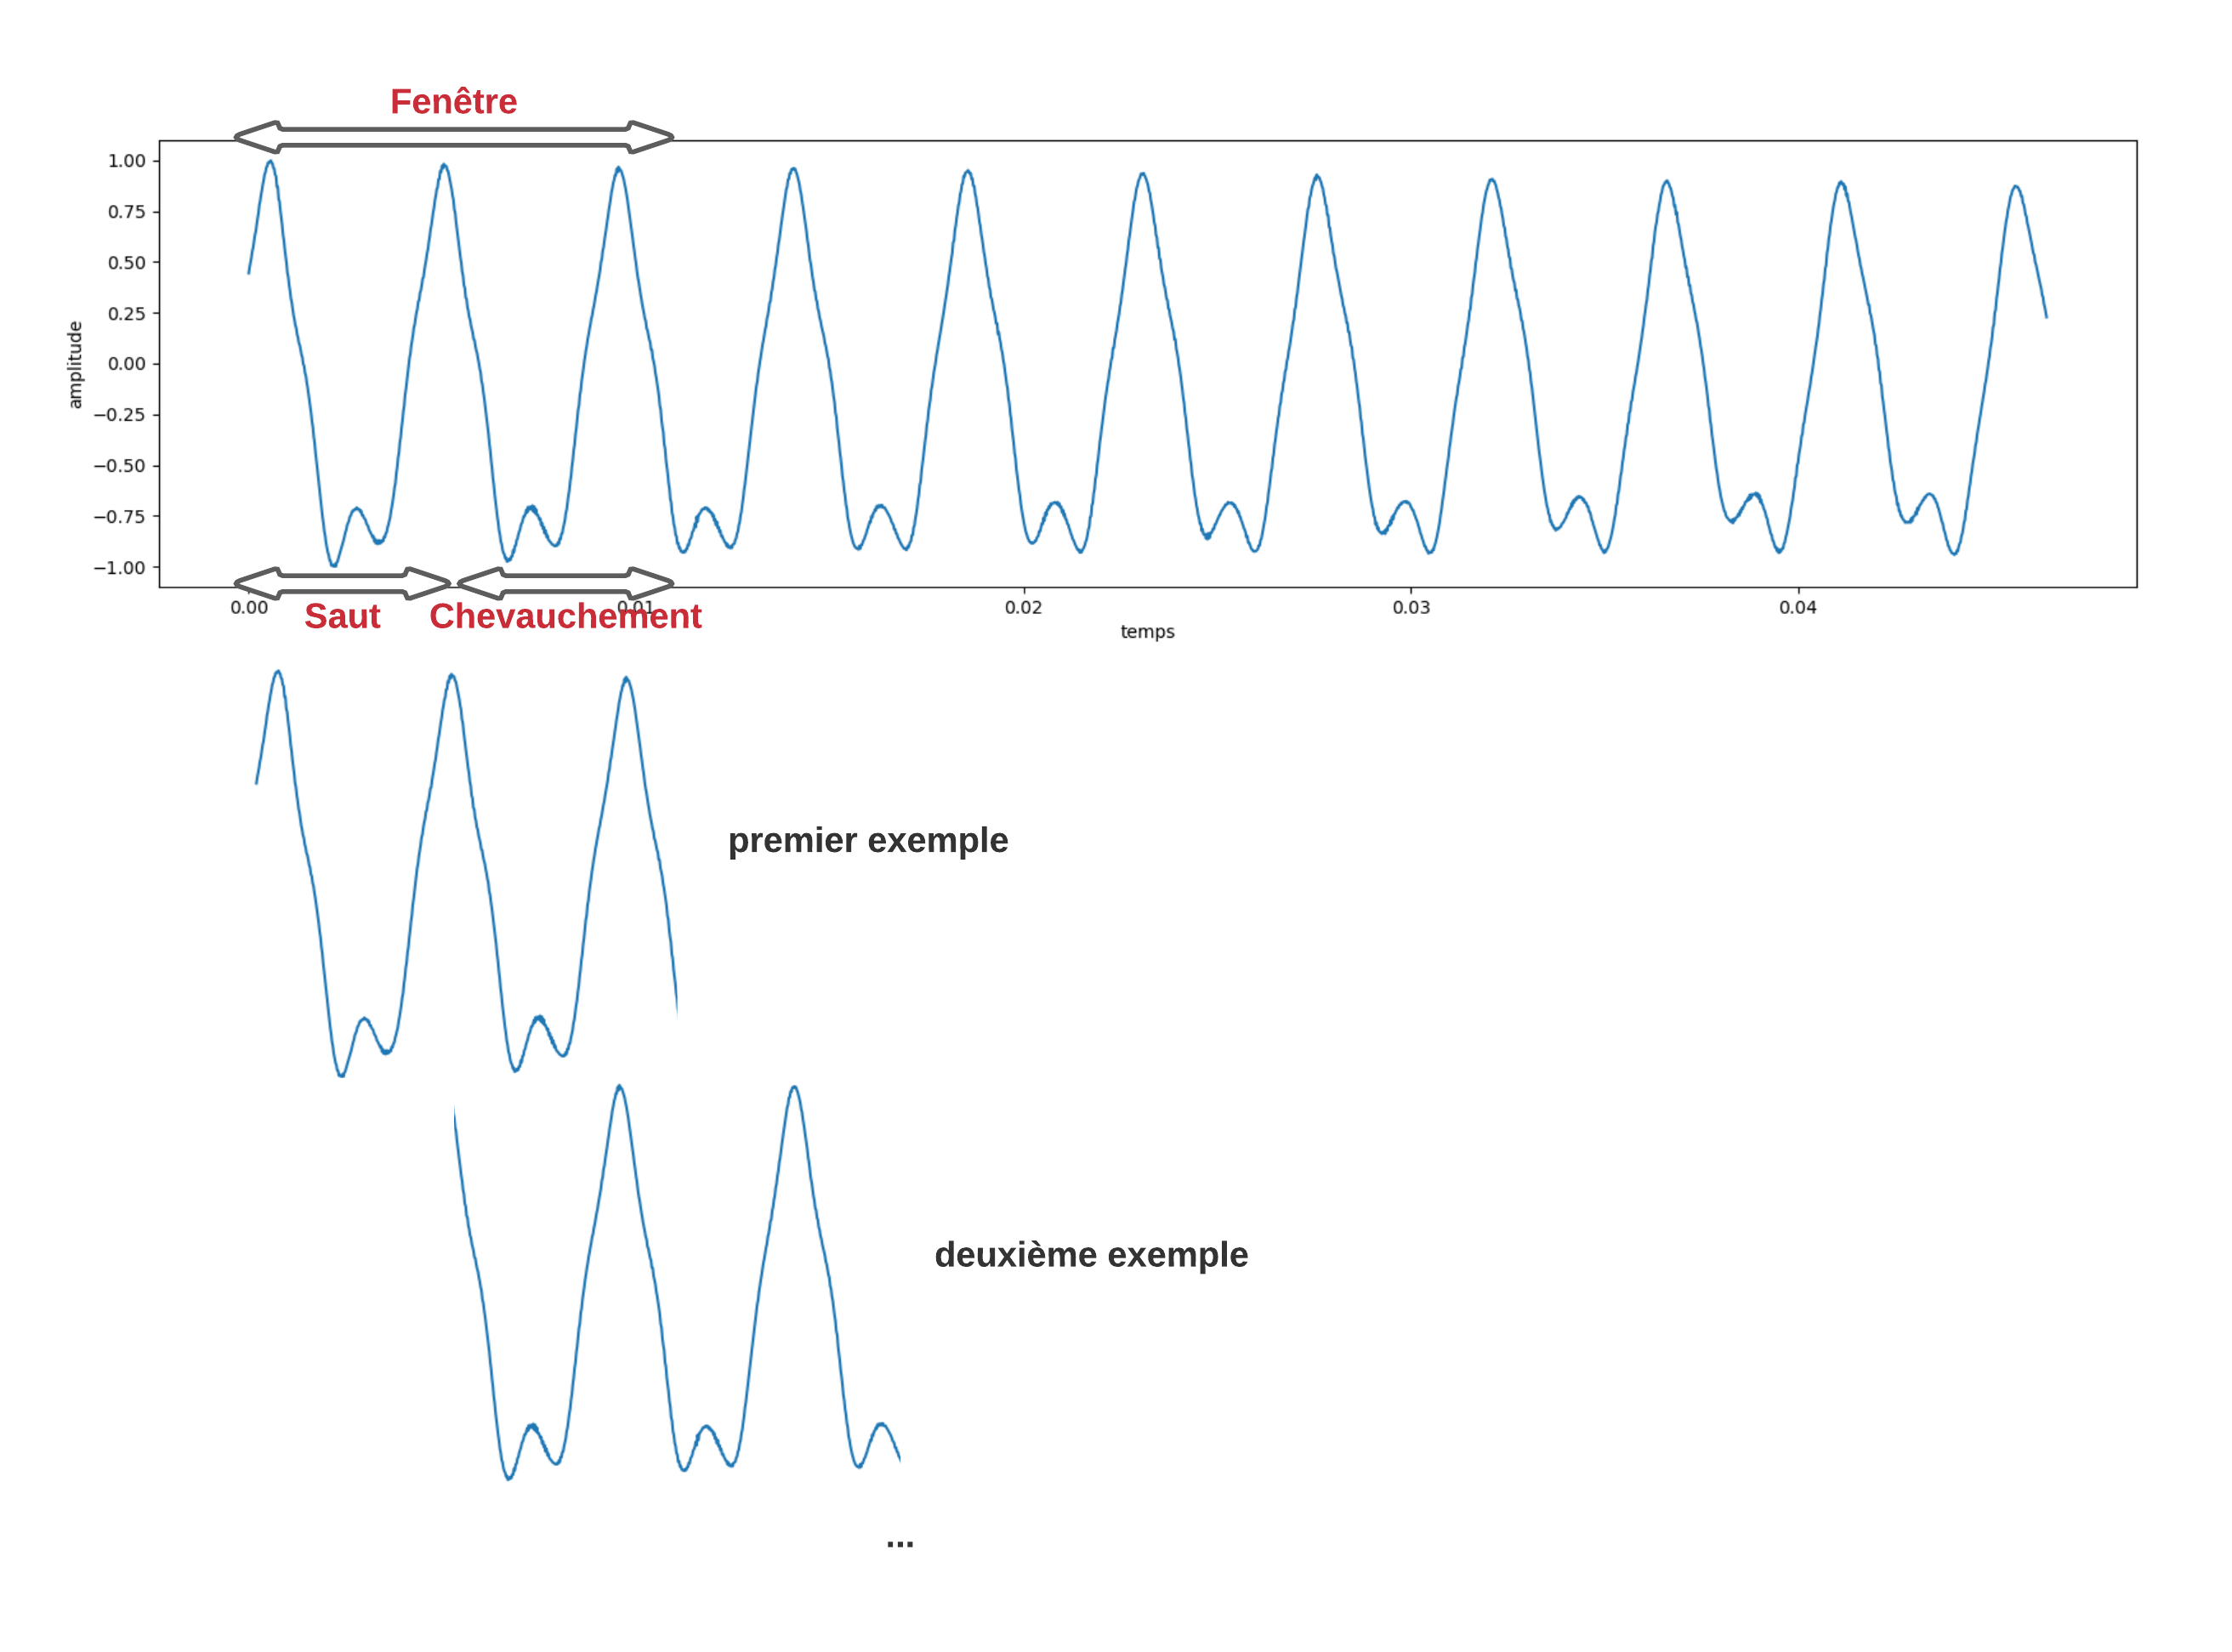
\includegraphics[width=1\linewidth]{signal_overlap}
	\caption[Chevauchement du signal]{Chevauchement du signal. Source : Réalisé par \textsc{Küenzi} Jean-Daniel. A partir de \textit{mathworks}, ref. URL10}
	\label{fig:signal_overlap}
\end{figure}

C'est une convention connue dans les analyses et traitements de série chronologique. Cela permet d'augmenter le nombre d'exemples et aussi de rendre le passage d'un exemple à un suivant beaucoup plus lisse sur l'axe x. Cela va contribuer à renforcer les modèles sur les changements de phase dans les signaux.

\subsection{Saut de l'attaque}

Finalement comme notre but est une utilisation en temps réel, l'attaque ne pose pas réellement de problème lors de la prédiction. Une attaque dure rarement plus que \textasciitilde0.02[s], donc lors de la prédiction en temps réel, elle sera à peine perceptive. En revanche elle va poser problème lors de l'entrainement du réseau. Comme elle contient beaucoup d'informations (bruit), si on essaye d'apprendre à classer l'attaque, cela va empêcher le réseau de converger correctement. Il est donc nécessaire de ne pas ajouter l'attaque dans nos exemples.

Pour ce faire, j'ai tout simplement décidé que le premier exemple valide de chaque signal était l'attaque et qu'il fallait l'ignorer. Ensuite pour ne pas retomber sur l'attaque lors du deuxième exemple, on se déplace directement sur l'axe x en utilisant la taille de la fenêtre et non la taille de saut.

\subsection{Taille de l'ensemble de données prétraité}

Le tableau ci-dessous, représente la taille de mon ensemble de données une fois qu'il est prétraité avec différentes tailles de fenêtres et donc de sauts. Une fois prétraité, l'ensemble de données sera réparti en lots (\textit{batches} en anglais) de 4'000 exemples.

\begin{table}[H]
	\centering{
		\begin{tabular}{c c l c }
			\hline
			\textbf{Nombre d'échantillons} & \textbf{Taille de saut} & \textbf{Données} & \textbf{Nombre d'exemples} \\
			\hline
			\multirow{2}{*}{1024} & \multirow{2}{*}{256} & Entrainement & 412'099 \\
			& & Validation & 254'564 \\
			\hline
			\multirow{2}{*}{2048} & \multirow{2}{*}{512} & Entrainement & 205'566 \\
			& & Validation & 127'019 \\
			\hline
			\multirow{2}{*}{3072} & \multirow{2}{*}{768} & Entrainement & 136'738 \\
			& & Validation & 84'516 \\
			\hline
			\multirow{2}{*}{4096} & \multirow{2}{*}{1024} & Entrainement & 102'347 \\
			& & Validation & 63'295 \\
			\hline
		\end{tabular}
		\caption[Taille de l'ensemble de données pour différentes tailles de fenêtres et de sauts]{Taille de l'ensemble de données pour différentes tailles de fenêtres et de sauts. Source : Réalisé par \textsc{Küenzi} Jean-Daniel}
		\label{tab:dataset}
	}
\end{table}